% Drawing 69/05-2 -- folder 69, batch 05, archive page 84 (PDF page 85).
% Transcription: Au milieu de la feuille, un grand dessin : un triangle dont les trois sommets sont marqués $\xi_{56}=\omega$ (en haut), $\xi_{12}=$ \ill{} (en bas à gauche) et $\xi_{34}=$ \ill{} (en bas à droite) ; de chacun part un éventail d'arêtes vers des sommets marqués d'indices doubles ou simples, primés ou non, certains cerclés, noircis ou encadrés. À gauche, les extrémités sont groupées par des accolades $a_1$, $a_2$, $a_3$, $a_4$ et portent notamment $\xi_1=\alpha_4$ \uncertain{}, $\xi'_2=\alpha'_1$, $\xi_{35}$, $\xi_{46}=\alpha'_3$ \uncertain{}, $\xi_{36}$, $\xi_{45}=\alpha_4$ ; en haut, les accolades $c_1$, \ldots, $c_4$, avec $\xi_{23}$, $\xi_{14}$, $\xi_{13}$, $\xi'_3$, $\xi_6$, $\xi'_6$, $\beta_1=\xi_5$ ; à droite et en bas, les accolades $b_1$, \ldots, $b_4$, avec $\beta_1$, $\beta_2$, $\beta_3$, $\beta_4$, $\xi_{51}$, $\xi_{52}$, $\xi_{26}$, $\xi_3$, $\xi_4$, $\xi'_3$, $\xi'_4$. Beaucoup d'indices, écrits serré et surchargés, se lisent mal.
% Kind: triangle with fans of edges grouped by braces. Method 2 (schematic redraw from the facsimile). Status: partial.
% Notes: The triangle xi_56 = omega (top), xi_12 (lower left), xi_34 (lower right), its three vertices placed once; from each vertex a fan of edges to its end vertices (seven at omega, eight at xi_12, eight at xi_34), every edge drawn from the vertex itself, so the fans meet exactly. End vertices as on the page: heavy dots, a box, open circles (the boxed and circled ones are drawn as rings); two ends of the omega fan are joined by short strokes, and two ends of the xi_34 fan. Labels: xi_56 = omega, xi_12, xi_34, the brace letters a_1 ... a_4 (left), c_1 ... c_4 and b_1, b_2 where they stand. Not drawn: the text column at the top left and the formulas a_1 + a_4 = alpha_1 .... The brace letters of the two other fans are c_1 ... c_4 and b_1 ... b_4 as the transcription reads them (settled 2026-11-12 by the mathematics): c_4, c_3, c_2, c_1 over the top fan, b_1 and b_2 under the right fan; b_3, b_4 lie beyond the crop, at the edge of the sheet. Redrawn 2026-11-09 (issue 128). Overlay check 2026-11-13 (claude-opus-5-5, issue 147): the 300 dpi colour rendering of the 250 ppi scan laid under the redraw, rasterised from its TikZ (not compiled: no TeX in the session): the triangle, the three fans and their end marks lie on their ink within 1 to 2 units (the earlier note's 2 to 3 units for the left fan no longer holds); nothing moved. Still differs: the small double indices at the fan ends (xi_23, xi_13, xi_6, ...) are mostly overwritten and stay left out; the braces are given by their letters only.
% Coordinates: 1 unit = 1 mm = 1/100 of the crop width (bbox in page fractions: [0.08, 0.06, 0.62, 0.47]).
% Redrawn by Claude (claude-opus-5-5), issue #73, 2026-11-09; not checked by a human; not compiled (no TeX in the session).
% Checked by Claude (claude-opus-5-5) 2026-11-13 (issue #147): overlaid on the colour scan (250 ppi, rendered at 300 dpi) and corrected; not compiled (no TeX in the session), rasterised for the overlay by a Python reader of this TikZ. Status: partial.
% Rights: reproduces part of the work -- behind RENDER_TRANSCRIPTS, never published by itself.
\documentclass[tikz,border=3pt]{standalone}
\usepackage{amsmath,amssymb}
\usetikzlibrary{patterns,arrows.meta}
\tikzset{pencil/.style={black!45}, struck/.style={black!35}, mpt/.style={circle,draw,inner sep=1.3pt}, pt/.style={circle,fill,inner sep=0.9pt}, opt/.style={circle,draw,fill=white,inner sep=1.1pt}}
\begin{document}
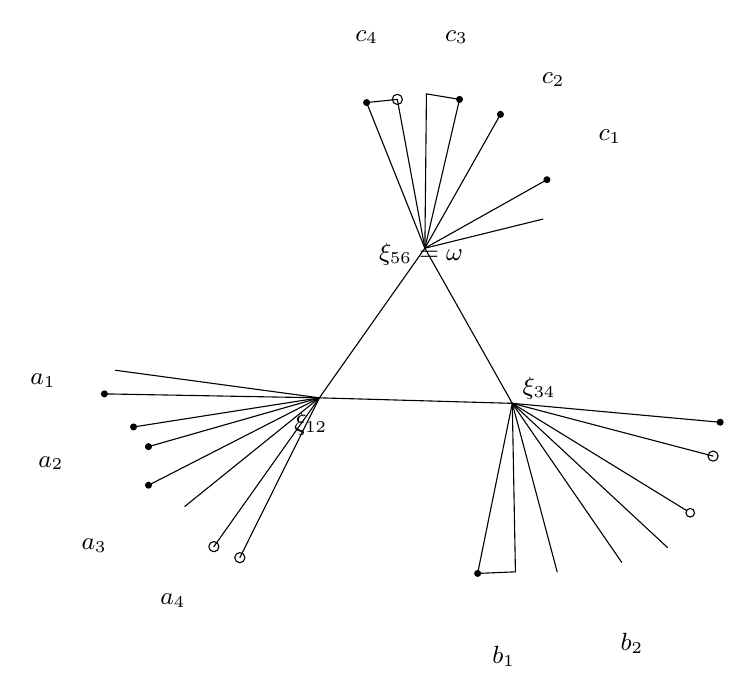
\begin{tikzpicture}[x=1mm,y=1mm,line cap=round,line join=round,font=\scriptsize]
\draw (61.5,-44.2) -- (48.1,-63.2) -- (72.6,-63.9) -- cycle;
\draw (61.5,-44.2) -- (54.1,-25.7);
\draw (61.5,-44.2) -- (58,-25.3);
\draw (61.5,-44.2) -- (61.7,-24.6);
\draw (61.5,-44.2) -- (65.9,-25.3);
\draw (61.5,-44.2) -- (71.1,-27.2);
\draw (61.5,-44.2) -- (77,-35.5);
\draw (61.5,-44.2) -- (76.5,-40.5);
\draw (48.1,-63.2) -- (22.2,-59.7);
\draw (48.1,-63.2) -- (20.8,-62.7);
\draw (48.1,-63.2) -- (24.5,-66.9);
\draw (48.1,-63.2) -- (26.4,-69.4);
\draw (48.1,-63.2) -- (26.4,-74.3);
\draw (48.1,-63.2) -- (31,-77);
\draw (48.1,-63.2) -- (34.7,-82.1);
\draw (48.1,-63.2) -- (38,-83.5);
\draw (72.6,-63.9) -- (99,-66.3);
\draw (72.6,-63.9) -- (98.1,-70.6);
\draw (72.6,-63.9) -- (95.2,-77.8);
\draw (72.6,-63.9) -- (92.3,-82.2);
\draw (72.6,-63.9) -- (86.5,-84.1);
\draw (72.6,-63.9) -- (78.3,-85.3);
\draw (72.6,-63.9) -- (73,-85.3);
\draw (72.6,-63.9) -- (68.2,-85.5);
\node[pt] at (54.1,-25.7) {};
\node[pt] at (65.9,-25.3) {};
\node[pt] at (71.1,-27.2) {};
\node[pt] at (77,-35.5) {};
\node[mpt] at (58,-25.3) {};
\draw (54.1,-25.7) -- (58,-25.3);
\draw (61.7,-24.6) -- (65.9,-25.3);
\node[pt] at (20.8,-62.7) {};
\node[pt] at (24.5,-66.9) {};
\node[pt] at (26.4,-69.4) {};
\node[pt] at (26.4,-74.3) {};
\node[mpt] at (34.7,-82.1) {};
\node[mpt] at (38,-83.5) {};
\node[pt] at (99,-66.3) {};
\node[mpt] at (98.1,-70.6) {};
\node[opt] at (95.2,-77.8) {};
\node[pt] at (68.2,-85.5) {};
\draw (73,-85.3) -- (68.2,-85.5);
\node[inner sep=1pt] at (61,-45) {\small $\xi_{56}=\omega$};
\node[inner sep=1pt] at (47,-66.5) {\small $\xi_{12}$};
\node[inner sep=1pt] at (76,-62) {\small $\xi_{34}$};
\node[inner sep=1pt] at (13,-61) {\small $a_1$};
\node[inner sep=1pt] at (14,-71.5) {\small $a_2$};
\node[inner sep=1pt] at (19.5,-82) {\small $a_3$};
\node[inner sep=1pt] at (29.5,-89) {\small $a_4$};
\node[inner sep=1pt] at (85,-30) {\small $c_1$};
\node[inner sep=1pt] at (77.8,-22.8) {\small $c_2$};
\node[inner sep=1pt] at (65.5,-17.4) {\small $c_3$};
\node[inner sep=1pt] at (54.1,-17.4) {\small $c_4$};
\node[inner sep=1pt] at (87.8,-94.4) {\small $b_2$};
\node[inner sep=1pt] at (71.5,-96) {\small $b_1$};
\end{tikzpicture}
\end{document}
